\documentclass[x11names]{article}
\usepackage[a4paper, total={6in, 9in}]{geometry}
\usepackage[skins]{tcolorbox}
\usepackage{tikz}
\usetikzlibrary{arrows}
\usetikzlibrary{calc}
\usepackage{pgfplots}
\pgfplotsset{compat=1.9}
\usepgflibrary{shapes.geometric}
\usepackage{xcolor}
\usepackage{amsmath}
\usepackage{fouriernc}
\usepackage{mathrsfs}
\usepackage{amssymb}
\usepackage{hyperref}

%% custom
\renewcommand*\contentsname{Indice}
\setcounter{tocdepth}{4}
\setcounter{secnumdepth}{2}
\pgfplotsset{compat=1.15}

% boxes
\definecolor{myblue}{RGB}{224, 245, 255} 
\definecolor{myred}{RGB}{234, 222, 255}
\definecolor{myorange}{RGB}{255, 102, 0}

\newtcolorbox{es}[2][]{%
	enhanced,colback=white,colframe=black,coltitle=black,
	sharp corners,boxrule=0.4pt,
	fonttitle=\itshape,frame style={dash pattern=on 3pt off 3pt},
	attach boxed title to top left={yshift=-0.5\baselineskip-0.4pt,xshift=2mm},
	boxed title style={tile,size=minimal,left=0.5mm,right=0.5mm,
		colback=white,before upper=\strut},
	title=#2,#1
}
\newtcolorbox{dym}[2][]{%
	enhanced,colback=white,colframe=black,coltitle=black,
	sharp corners,boxrule=0.4pt,
	fonttitle=\itshape,,
	attach boxed title to top left={yshift=-0.5\baselineskip-0.4pt,xshift=2mm},
	boxed title style={tile,size=minimal,left=0.5mm,right=0.5mm,
		colback=white,before upper=\strut},
	title=#2,#1
}
\newtcolorbox{blues}[2][]{%
	enhanced,colback=myblue,colframe=black,coltitle=black,
	sharp corners,boxrule=0.4pt,
	fonttitle=\bfseries\itshape,
	attach boxed title to top left={yshift=-0.5\baselineskip-0.4pt,xshift=2mm},
	boxed title style={tile,size=minimal,left=0.5mm,right=0.5mm,
		colback=myblue,before upper=\strut},
	title=#2,#1
}
\newtcolorbox{redes}[2][]{%
	enhanced,colback=myred,colframe=black,coltitle=black,
	sharp corners,boxrule=0.4pt,
	fonttitle=\bfseries\itshape,
	attach boxed title to top left={yshift=-0.5\baselineskip-0.4pt,xshift=2mm},
	boxed title style={tile,size=minimal,left=0.5mm,right=0.5mm,
		colback=myred,before upper=\strut},
	title=#2,#1
}


\newcommand*{\QEDA}{\null\nobreak\hfill\ensuremath{\blacksquare}}%
\newcommand*{\QEDB}{\null\nobreak\hfill\ensuremath{\square}}%

\newcommand{\esempio}[2]{
	\begin{es}{esempio #1}
		#2
	\end{es}
}
\newcommand{\definizione}[2]{
	\begin{center}
		\fboxsep11pt
		\colorbox{myblue}{\begin{minipage}{5.75in}
				\begin{blues}{Definizione: #1}
					#2
				\end{blues}
		\end{minipage}}
	\end{center}
}
\newcommand{\teorema}[2]{
	\begin{center}
		\fboxsep11pt
		\colorbox{myred}{\begin{minipage}{5.75in}
				\begin{redes}{#1}
					#2
				\end{redes}
		\end{minipage}}
	\end{center}
}
\newcommand{\dimostrazione}[2]{
	\begin{dym}{dimostrazione: #1}
		#2
		\QEDB
	\end{dym}
}

\pgfplotsset{my axis/.append style={height=9cm,width=9cm,grid=major,samples=100,yticklabel=\empty,xticklabel=\empty}}
\pgfplotsset{my plot/.append style={thick,samples=500}}

\begin{document}
	
\begin{titlepage}
   \begin{center}
       \vspace*{1cm}
        
       \textbf{\LARGE Relazione di laboratorio - Esperienza di Poisson}
       
       \vspace{0.3cm}
       \large \textit{Rate di una sorgente radioattiva} \\
       
       \vspace{0.5cm}
       \Large Federico Cesari \\
       
       \small 1096759

			
		\vspace{1cm}
		\begin{center}
			\includegraphics[scale=1.2]{geiger.jpeg}	
		\end{center}
		
		

       \vfill
            
       
            
       \vspace{0.8cm}
     
       
            
       corso A\\
       Università degli studi di Torino, Torino\\
       3 marzo 2024\\
       
            
   \end{center}
\end{titlepage}

\tableofcontents
\newpage
	
	
\section{Successioni di funzioni}

\begin{center}
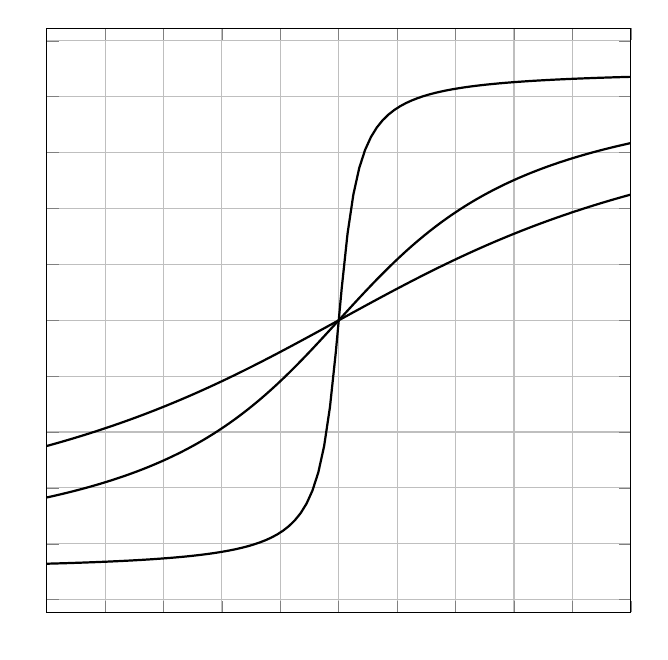
\begin{tikzpicture}
	\begin{axis}[my axis,xmin=-1,xmax=1]
		\addplot[my plot, domain y=-pi/2:pi/2] {atan(x)};
		\addplot[my plot, domain y=-pi/2:pi/2] {atan(2*x)};
		\addplot[my plot, domain y=-pi/2:pi/2] {atan(20*x)};
	\end{axis}
\end{tikzpicture}
\end{center}

\subsection{Limiti di successioni}


\definizione{Convergenza puntuale}{}

\definizione{Convergenza uniforme}{}


\esempio{1}{}
\esempio{2}{}
\esempio{3}{}



\teorema{Teorema 1}{}
\dimostrazione{}{}

\teorema{Teorema 2}{}
\dimostrazione{}{}

\esempio{4}{}

\teorema{Teorema}{}


% SERIE DI FUNZIONI
\section{Serie di funzioni}
Presa \((f_{n})_{n}\) successione di funzioni, \(f_{n}:A\subseteq \mathbb{R} \to \mathbb{R}\) (o \(\mathbb{C}\)), chiamiamo \textbf{serie di funzioni}, indicata con
\[ 
\sum_n f_{n}(x)
\]
la successione delle ridotte 
\[ 
S_{N} = \sum_{n=1}^N f_{n}(x)
\]
\paragraph{Convergenza della serie} Diciamo che la serie converge (puntualmente o uniformemente) su un insieme \(E\subseteq A\) se lo fa la successione delle ridotte. Si andrà quindi a studiare il limite di \(S_{N}\) che chiamiamo somma della serie.

\teorema{Teorema 1S}{
Data \(f:A\subseteq \mathbb{R} \to \mathbb{R}\), se
\begin{itemize}
	\item \(f_{n}\) continue su \(E\subseteq A\);
	\item \(\sum_n f_{n}\) converge uniformemente su \(E\subseteq A\) alla somma \(S(x)\)
\end{itemize}
Allora \(S(x)\) è continua su \(E\).}
\teorema{Teorema 2S}{
Data \(f:A\subseteq \mathbb{R} \to \mathbb{R}\) e \(E = [a,b]\subseteq \mathbb{R}\), se
\begin{itemize}
\item \(f_{n}\) continue su \(E\subseteq A\);
\item \(\sum_n f_{n}\) converge uniformemente su \(E\subseteq A\) alla somma \(S(x)\)
\end{itemize}
Allora
\[ 
\int_{a}^{b} \sum f_{n}(x)dx \quad  = \quad \sum \int_{a}^{b}  f_{n}(x)dx 
\]}

\definizione{}{
	\[ 
	I_{s} = \left\{x \;\:\;\ \text{la serie considerata} \sum f_{n}(x) \text{converge semplicemente} \right\}
	\]
	per la serie \(\sum x^n\) si ha che \(I_{s} = (-1,1)\)
	\[ 
	I_{a} = \left\{x \;\:\;\ \text{la serie considerata} \sum |f_{n}(x)| \text{converge semplicemente} \right\}
	\]
}

\teorema{Teorema: m-test o criterio di convergenza totale}{
Date 
\begin{itemize}
	\item \((f_{n})_{n}\) successione di funzioni su \(E\subseteq \mathbb{R}\) (o in \(\mathbb{C}\));
	\item \((m_{n})_{n} \subseteq \mathbb{R}\) successione di numeri reali positivi. 
\end{itemize}
tali che
\begin{itemize}
	\item \((H_{1})\qquad\) \(|f_{n}(x)|\leq m_{n}\) \(\forall x \in E\), \(\forall n\);
	\item \((H_{2})\qquad\) \(\sum m_{n}(x) < + \infty\).
\end{itemize}
Allora la serie \(\sum f_{n}(x)\) converge assolutamente in ongi punto di \(E\) è uniformemente su \(E\) \(\implies\) la serie converge totalmente.
}




	
\end{document}